\documentclass[12pt,a4paper]{article}  % Déclare la classe du document.

\newcommand{\chaptermark}[2]{\og #2 \fg{} (#1)} % ligne uniquement pour éviter une erreur en cas d'article
\usepackage[table,dvipsnames,svgnames]{xcolor}
\usepackage{listingsutf8}
%\usepackage[utf8]{inputenc}% gestion des accents (source)
\usepackage[T1]{fontenc}% gestion des accents (PDF)
\usepackage{fontspec}
\usepackage[french]{babel}% gestion du français
\usepackage{textcomp}% caractères additionnels
\usepackage{mathtools,amssymb,amsthm}% packages de l'AMS + mathtools
\usepackage{amsmath}
\usepackage{yhmath}
\usepackage{mathpazo}
\usepackage[scaled=0.95]{helvet}
\usepackage{courier}
%\usepackage{fourier}
%\usepackage[scaled=0.95]{helvet}
%\usepackage{courier}
\usepackage{bm}
\usepackage{gensymb}
\usepackage{graphicx}

\usepackage{enumitem}
\usepackage{pifont}

\usepackage{pstricks}
\usepackage{pstricks-add}
\usepackage{pst-eucl}
\usepackage{pgfplots}
\let\clipbox\relax
%\usepackage{pst-plot,pst-text,pst-tree,pstricks-add}
%\usepackage{pst-node} % required package
\usepackage{pst-all}
\usepackage[most,skins,breakable]{tcolorbox}

\usepackage{euscript}





% ############### Nouvelles commandes ###############
% Coloration des labels des points dans pst-eucl
\makeatletter
\define@key[psset]{pst-eucl}{LabelColor}{\def\psk@LabelColor{#1}}
\psset{LabelColor=black}
\def\Pst@WhichLabel#1{{\color{\psk@LabelColor}%
		\ifx\psk@PointName\@default#1\else\psk@PointName\fi}}
\makeatother

% renomme le symbole #2 en #1#2 et invalide le symbole initial #2:
\def\renamesymbol#1#2{
	\expandafter\let\expandafter\newsym\expandafter=\csname#2\endcsname
	\expandafter\global\expandafter\let\csname#1#2\endcsname=\newsym
	\expandafter\global\expandafter\let\csname#2\endcsname=\origsym
}



\usepackage{ProfCollege}
\renamesymbol{Casio}{Calculatrice}
\usepackage[nonshellescape]{ProfLycee}



%\usepackage[left=1.5cm,right=1.5cm,top=2.5cm,bottom=2.5cm]{geometry}
\usepackage[left=13mm,right=13mm,top=18mm,bottom=18mm,footskip=30pt]{geometry}
\setlength{\headheight}{15pt}

\usepackage{titlesec}
\usepackage{pas-math}
\usepackage{longtable}
\usepackage{tikz,tkz-tab}
\usepackage{amsmath}
\usepackage[right]{eurosym}
\usepackage{sectsty}
\usepackage{tipfr}
\usepackage{setspace}

%pour faire les touches de la calculatrices
\usepackage{menukeys}
\renewmenumacro{\menu}{roundedmenus} % default: menus
\renewmenumacro{\directory}{pathswithfolder} % default: paths
\renewmenumacro{\keys}{shadowedroundedkeys} % default: roundedkeys


\usepackage{multicol}
\usepackage{multirow}
\usepackage{systeme}

%% Format des titres de chapitres, paragraphes, ...
\titleformat{\chapter}[frame]
{\color{red!85!white}\normalsize}%
{\filright\sffamily\Large%
	\enspace Chapitre \thechapter\enspace}%
{8pt}
{\color{red!85!white}\rule{0pt}{30pt}\sffamily\Huge\bfseries\filcenter}
%%%%%%%%%%%%%%%%%%%%
\titlespacing{\chapter}{0pc}{0pc}{2pc}
\titlespacing{\subsection}{2pc}{}{}

\titleformat{\subsection}[block]{\hspace{1em}}{\thesubsection}{1em .}{}
\titleformat{\subsubsection}[block]{\hspace{2em}}{\thesubsection}{1em )}{}

\chapterfont{\color{red}{}}
\sectionfont{\color{green!55!black}{}}
\subsectionfont{\color{cyan!65!black}{}}
\subsubsectionfont{\color{violet}{}}
\renewcommand{\thesection}{\color{green!55!black}\Roman{section}.}
\renewcommand{\thesubsection}{\color{cyan!65!black}\arabic{subsection})}
\renewcommand{\thesubsubsection}{\color{violet}\alph{subsubsection})}
\setcounter{secnumdepth}{3}

\titleformat{\subsection}[block]{\hspace{1em}}{\thesubsection}{1em .}{}
\titleformat{\subsubsection}[block]{\hspace{2em}}{\thesubsection}{1em )}{}

\usepackage[column=A]{cellspace}
\setlength{\cellspacebottomlimit}{4pt}
\setlength{\cellspacetoplimit}{4pt}
\setlength{\parindent}{2pt}
\setlength{\tabcolsep}{0.5cm}


%entête et pieds de pages
\usepackage{fancyhdr}
\pagestyle{fancy}
\fancyhf{}
\usepackage{lastpage}
\renewcommand{\chaptermark}[1]{\markboth {Chap. \thechapter~ - ~#1}{}}
\renewcommand\headrulewidth{1pt}
\fancyhead[LO,RE]{1ère G - spécialité maths}
\fancyhead[RO,LE]{\leftmark}
\renewcommand\footrulewidth{1pt}
\fancyfoot[LO,RE]{Année 2025-2026}
\fancyfoot[RO,LE]{\textbf{Page \thepage/\pageref{LastPage}}}

%Mes boites pour les définitions, propriétés, remarques, ...

%Mes boites pour les définitions, propriétés, remarques, ...

\newcommand\titrebox[1]{\textbf{#1}}
\newtcolorbox{definition}{breakable,colback=red!10!white,
	colframe=red!85!white, fonttitle=\bfseries,enhanced,
	attach boxed title to top left={xshift=5mm, yshift=-2mm},boxed title style={size=small,colback=red!10!white,colframe=red!85!white, arc=0.5mm},
	title=\textcolor{red!85!white}{Définition} , arc=3mm}

\newtcolorbox{definitionTitre}[1]{breakable,colback=red!10!white,
	colframe=red!85!white, fonttitle=\bfseries,enhanced,
	attach boxed title to top left={xshift=5mm, yshift=-2mm},boxed title style={size=small,colback=red!10!white,colframe=red!85!white, arc=0.5mm},
	title=\textcolor{red!85!white}{Définition - #1} , arc=3mm}

\newtcolorbox{definitionPerso}[1]{breakable,colback=red!10!white,
	colframe=red!85!white, fonttitle=\bfseries,enhanced,
	attach boxed title to top left={xshift=5mm, yshift=-2mm},boxed title style={size=small,colback=red!10!white,colframe=red!85!white, arc=0.5mm},
	title=\textcolor{red!85!white}{#1} , arc=3mm}

\newtcolorbox{regle}{breakable,colback=red!10!white,
	colframe=red!85!white, fonttitle=\bfseries,enhanced,
	attach boxed title to top left={xshift=5mm, yshift=-2mm},boxed title style={size=small,colback=red!10!white,colframe=red!85!white, arc=0.5mm},
	title=\textcolor{red!85!white}{Règle} , arc=3mm}

\newtcolorbox{regles}{breakable,colback=red!10!white,
	colframe=red!85!white, fonttitle=\bfseries,enhanced,
	attach boxed title to top left={xshift=5mm, yshift=-2mm},boxed title style={size=small,colback=red!10!white,colframe=red!85!white, arc=0.5mm},
	title=\textcolor{red!85!white}{Règles} , arc=3mm}

\newtcolorbox{definitions}{breakable,colback=red!10!white,
	colframe=red!85!white, fonttitle=\bfseries,enhanced,
	attach boxed title to top left={xshift=5mm, yshift=-2mm},boxed title style={size=small,colback=red!10!white,colframe=red!85!white, arc=0.5mm},
	title=\textcolor{red!85!white}{Définitions} , arc=3mm}

\newtcolorbox{propriete}{breakable,colback=red!10!white,
	colframe=red!85!white, fonttitle=\bfseries,enhanced,
	attach boxed title to top left={xshift=5mm, yshift=-2mm},boxed title style={size=small,colback=red!10!white,colframe=red!85!white, arc=0.5mm},
	title=\textcolor{red!85!white}{Propriété} , arc=3mm}

\newtcolorbox{proprieteTitre}[1]{breakable,colback=red!10!white,
	colframe=red!85!white, fonttitle=\bfseries,enhanced,
	attach boxed title to top left={xshift=5mm, yshift=-2mm},boxed title style={size=small,colback=red!10!white,colframe=red!85!white, arc=0.5mm},
	title=\textcolor{red!85!white}{Propriété - #1} , arc=3mm}

\newtcolorbox{proprietes}{breakable,colback=red!10!white,
	colframe=red!85!white, fonttitle=\bfseries,enhanced,
	attach boxed title to top left={xshift=5mm, yshift=-2mm},boxed title style={size=small,colback=red!10!white,colframe=red!85!white, arc=0.5mm},
	title=\textcolor{red!85!white}{Propriétés} , arc=3mm}

\newtcolorbox{theoreme}{breakable,colback=red!10!white,
	colframe=red!85!white, fonttitle=\bfseries,enhanced,
	attach boxed title to top left={xshift=5mm, yshift=-2mm},boxed title style={size=small,colback=red!10!white,colframe=red!85!white, arc=0.5mm},
	title=\textcolor{red!85!white}{Théorème} , arc=3mm}

\newtcolorbox{theoremeTitre}[1]{breakable,colback=red!10!white,
	colframe=red!85!white, fonttitle=\bfseries,enhanced,
	attach boxed title to top left={xshift=5mm, yshift=-2mm},boxed title style={size=small,colback=red!10!white,colframe=red!85!white, arc=0.5mm},
	title=\textcolor{red!85!white}{Théorème - #1} , arc=3mm}

\newtcolorbox{theoremes}{breakable,colback=red!10!white,
	colframe=red!85!white, fonttitle=\bfseries,enhanced,
	attach boxed title to top left={xshift=5mm, yshift=-2mm},boxed title style={size=small,colback=red!10!white,colframe=red!85!white, arc=0.5mm},
	title=\textcolor{red!85!white}{Théorèmes} , arc=3mm}

\newtcolorbox{bexemple}{
	enhanced,
	breakable,
	fonttitle=\bfseries,
	frame empty,
	nobeforeafter,
	borderline west={0.5mm}{0mm}{cyan!75!black},
	title=\textcolor{cyan!75!black}{\faHubspot\:\:Exemple},
	%title after break=Exemple (suite),
	colback=white,
	extras={enhanced, frame empty},
	detach title,before upper={\tcbtitle\ :\quad },
}

\newtcolorbox{bexemples}{
	enhanced,
	breakable,
	fonttitle=\bfseries,
	frame empty,
	nobeforeafter,
	borderline west={0.5mm}{0mm}{cyan!75!black},
	title=\textcolor{cyan!75!black}{\faHubspot\:\:Exemples},
	%title after break=Exemples (suite),
	colback=white,
	extras={enhanced, frame empty},
	detach title,before upper={\tcbtitle\ :\quad },
}

\newtcolorbox{bexemplet}[1]{
	enhanced,
	breakable,
	fonttitle=\bfseries,
	frame empty,
	borderline west={0.5mm}{0mm}{cyan!75!black},
	title=\textcolor{cyan!75!black}{\faHubspot\:\:Exemple - #1},
	colback=white,
	extras={enhanced, frame empty},
	detach title,before upper={\tcbtitle\ :\quad },
}

\newtcolorbox{brmq}{
	enhanced,
	breakable,
	fonttitle=\bfseries,
	frame empty,
	nobeforeafter,
	borderline west={0.5mm}{0mm}{orange!95!white},
	title=\textcolor{orange!85!white}{\faHandPointRight[regular]\:\:Remarque} ,
	colback=white,
	extras={enhanced, frame empty},
	detach title,before upper={\tcbtitle\ \quad },
}

\newtcolorbox{brmqs}{
	enhanced,
	breakable,
	fonttitle=\bfseries,
	frame empty,
	nobeforeafter,
	borderline west={0.5mm}{0mm}{orange!85!white},
	title=\textcolor{orange!85!white}{\faHandPointRight[regular]\:\:Remarques},
	colback=white,
	detach title,before upper={\tcbtitle\ \quad },
	extras={enhanced, frame empty},
}

\newtcolorbox{brmqt}[1]{
	enhanced,
	breakable,
	fonttitle=\bfseries,
	frame empty,
	nobeforeafter,
	borderline west={0.5mm}{0mm}{orange!85!white},
	title=\textcolor{orange!85!white}{\faHandPointRight[regular]\:\:Remarque - #1},
	colback=white,
	extras={enhanced, frame empty},
	detach title,before upper={\tcbtitle\ \quad },
}

\newtcolorbox{consequences}[1]{
	enhanced,
	breakable,
	fonttitle=\bfseries,
	frame empty,
	nobeforeafter,
	borderline west={0.5mm}{0mm}{ProcessBlue},
	title=\textcolor{ProcessBlue}{#1},
	colback=white,
	extras={enhanced, frame empty},
	detach title,before upper={\tcbtitle\ :\quad },
}

\newtcolorbox{bmethode}{
	enhanced,
	breakable,
	fonttitle=\bfseries,
	frame empty,
	nobeforeafter,
	borderline west={0.5mm}{0mm}{blue!75!black},
	title=\textcolor{blue!75!black}{Méthode} ,
	colback=white,
	extras={enhanced, frame empty},
	attach boxed title to top left = {xshift = -3mm},
	boxed title style={size=small,colback=white,colframe=blue!75!black, arc=3mm,
	}
}

\newtcolorbox{bmethodes}{
	enhanced,
	breakable,
	fonttitle=\bfseries,
	frame empty,
	nobeforeafter,
	borderline west={0.5mm}{0mm}{blue!75!black},
	title=\textcolor{blue!75!black}{Méthodes} ,
	colback=white,
	extras={enhanced, frame empty},
	attach boxed title to top left = {xshift = -3mm},
	boxed title style={size=small,colback=blue!75!black,colframe=blue!75!black, arc=3mm,
	}
	boxed title after break style={size=small,colback=white,colframe=blue!75!black, arc=3mm,
	}
}

\newtcolorbox{bmethodet}[1]{
	enhanced,
	breakable,
	fonttitle=\bfseries,
	frame empty,
	nobeforeafter,
	borderline west={0.5mm}{0mm}{blue!75!black},
	title=\textcolor{blue!75!black}{\faTasks\:\:Méthode - #1} ,
	colback=white,
	extras={enhanced, frame empty},
	attach boxed title to top left = {xshift = -3mm},
	boxed title style={size=small,colback=white,colframe=blue!75!black, arc=3mm,
	}
}

\newtcolorbox{bdemo}{
	enhanced,
	breakable,
	fonttitle=\bfseries,
	frame empty,
	nobeforeafter,
	borderline west={0.5mm}{0mm}{violet!65!white},
	title={\faEdit[regular]\:\:Démonstration},
	%title after break=Démonstration (suite),
	colback=white,
	extras={enhanced, frame empty},
	attach boxed title to top left = {xshift = -3mm},
	boxed title style={size=small,colback=violet!65!white,colframe=violet!65!white, arc=3mm,
	}
}

\newtcolorbox{bdemos}{
	enhanced,
	breakable,
	fonttitle=\bfseries,
	frame empty,
	nobeforeafter,
	borderline west={0.5mm}{0mm}{violet!65!white},
	title={\faEdit[regular]\:\:Démonstrations},
	%title after break=Démonstration (suite),
	colback=white,
	extras={enhanced, frame empty},
	attach boxed title to top left = {xshift = -3mm},
	boxed title style={size=small,colback=violet!65!white,colframe=violet!65!white, arc=3mm,
	}
}

\newtcolorbox{bdemot}[1]{
	enhanced,
	breakable,
	fonttitle=\bfseries,
	frame empty,
	nobeforeafter,
	borderline west={0.5mm}{0mm}{violet!65!white},
	title={\faEdit[regular]\:\:Démonstration - #1},
	%title after break=Démonstration (suite),
	colback=white,
	extras={enhanced, frame empty},
	attach boxed title to top left = {xshift = -3mm},
	boxed title style={size=small,colback=violet!65!white,colframe=violet!65!white, arc=3mm,
	}
}

\newtcolorbox{boxPerso}[2]{
	enhanced,
	breakable,
	fonttitle=\bfseries,
	frame empty,
	nobeforeafter,
	borderline west={0.5mm}{0mm}{#2},
	title=#1,
	%title after break=Exemple (suite),
	colback=white,
	extras={enhanced, frame empty},
	detach title,before upper={\tcbtitle\ :\quad },
}


\newcommand*{\Coord}[3]{% 
	\ensuremath{\vv{#1}\, 
		\begin{pmatrix} 
			#2\\ 
			#3 
\end{pmatrix}}}

\newcommand*{\CoordSV}[2]{% 
	\ensuremath{\begin{pmatrix} 
			#1\\ 
			#2 
\end{pmatrix}}}

\newcommand*{\Coordp}[3]{% 
	\ensuremath{\vv{#1}\, 
		\left\lvert 
		\begin{matrix} 
			#2\\ 
			#3 
		\end{matrix}  
		\right.% Ne pas oublier le délimiteur invisible. 
}}


%personnalisation des listes non numérotées pour les différentes boites 
\newlist{itemEx}{itemize}{2}
\setlist[itemEx,1]{label=$\bullet$, font=\color{cyan!75!black}}
\setlist[itemEx,2]{label=$\bullet$, font=\color{cyan!75!black}}

\newlist{enumEx}{enumerate}{2}
\setlist[enumEx,1]{label=\arabic*), font=\bf\color{cyan!75!black}}
\setlist[enumEx,2]{label=\alph*), font=\bf\color{cyan!75!black}}

\newlist{itemMet}{itemize}{2}
\setlist[itemMet,1]{label=$\bullet$, font=\color{blue!75!black}}
\setlist[itemMet,2]{label=$\bullet$, font=\color{blue!75!black}}

\newlist{enumMet}{enumerate}{2}
\setlist[enumMet,1]{label=\arabic*), font=\bf\color{blue!75!black}}
\setlist[enumMet,2]{label=\alph*), font=\bf\color{blue!75!black}}

\newlist{itemDef}{itemize}{2}
\setlist[itemDef,1]{label=$\bullet$, font=\color{ForestGreen}}
\setlist[itemDef,2]{label=$\bullet$, font=\color{ForestGreen}}

\newlist{enumDef}{enumerate}{2}
\setlist[enumDef,1]{label=\arabic*), font=\bf\color{ForestGreen}}
\setlist[enumDef,2]{label=\alph*), font=\bf\color{ForestGreen}}

\newlist{itemProp}{itemize}{2}
\setlist[itemProp,1]{label=$\bullet$, font=\color{red!85!white}}
\setlist[itemProp,2]{label=$\bullet$, font=\color{red!85!white}}

\newlist{enumProp}{enumerate}{2}
\setlist[enumProp,1]{label=\arabic*), font=\bf\color{red!85!white}}
\setlist[enumProp,2]{label=\alph*), font=\bf\color{red!85!white}}

\newlist{itemDem}{itemize}{2}
\setlist[itemDem,1]{label=$\bullet$, font=\color{violet!85!white}}
\setlist[itemDem,2]{label=$\bullet$, font=\color{violet!85!white}}

\newlist{enumDem}{enumerate}{2}
\setlist[enumDem,1]{label=\arabic*), font=\bf\color{violet!85!white}}
\setlist[enumDem,2]{label=\alph*), font=\bf\color{violet!85!white}}

\newlist{itemRem}{itemize}{2}
\setlist[itemRem,1]{label=\ding{43}, font=\color{orange!85!white}}
\setlist[itemRem,2]{label=\ding{43}, font=\color{orange!85!white}}

\newlist{enumRem}{enumerate}{2}
\setlist[enumRem,1]{label=\arabic*), font=\bf\color{orange!85!white}}
\setlist[enumRem,2]{label=\alph*), font=\bf\color{orange!85!white}}

% nouvelle commande pour mettre entre guillemets une expression
\newcommand{\guillemets}[1]{\og \emph{#1} \fg}


\newcommand{\corr}[1]{\fcolorbox{red}{yellow!30}{#1}}

\newtcolorbox{corrBox}{enhanced,breakable,boxrule=1pt,nobeforeafter,boxsep=0pt,left=\fboxsep,right=\fboxsep,colback=yellow!30,colframe=red!75!black}

% commandes pour mettre en couleur (et en gras) dans une expression mathématique.
\newcommand{\mVert}[1]{{\color{green!55!black}\bm{#1}}}
\newcommand{\mVertWB}[1]{{\color{green!55!black}#1}}
\newcommand{\mRouge}[1]{{\color{red!85!white}\bm{#1}}}
\newcommand{\mRougeWB}[1]{{\color{red!85!white}#1}}
\newcommand{\mBleu}[1]{{\color{blue!75!black}\bm{#1}}}
\newcommand{\mBleuWB}[1]{{\color{blue!75!black}#1}}
\newcommand{\mOrange}[1]{{\color{orange!75!white}\bm{#1}}}
\newcommand{\mOrangeWB}[1]{{\color{orange!75!white}#1}}
\newcommand{\mViolet}[1]{{\color{violet!85!white}\bm{#1}}}
\newcommand{\mVioletWB}[1]{{\color{violet!85!white}#1}}

%commandes pour les flèches de distributivité.
\newcommand{\tikzmarkBB}[2][]{ \tikz[remember picture, overlay, baseline=-0.5ex]\node[#1, left](#2){}; }
\newcommand{\flechePropV}[4][]{ \tikz[remember picture, overlay]\draw (#2)edge[bend left=90,min distance=1em, -stealth]node[midway, #1]{#4}(#3); }
\newcommand{\flechePropH}[4][]{ \tikz[remember picture, overlay]\draw (#2)edge[bend left=90, min distance=1em, -stealth]node[midway, #1]{#4}(#3); }
\newcommand{\flechePropHbas}[4][]{ \tikz[remember picture, overlay]\draw (#2)edge[bend left=-90, min distance=1em, -stealth]node[midway, #1]{#4}(#3); }


\lstdefinestyle{algo}{%
	inputencoding=utf8,
	mathescape,
	basicstyle=\footnotesize\ttfamily,
	numberstyle=\scriptsize\ttfamily\color{gray},
	showstringspaces=false,
	tabsize=2,
	numbers=left,
	framexleftmargin=8mm,
	xleftmargin=8mm,
	keepspaces=true,
	frame=lines,
	framerule=1pt,
	rulecolor=\color{green!50!black},
	backgroundcolor=\color{green!5},
	keywords = {Pour, allant, Si, alors, Sinon, Fin},    
	morecomment=[l][commentstyle]{//},
	commentstyle=\color{gray},
	classoffset=0,
	keywordstyle=\color{blue!75},
	classoffset=1,
	morekeywords = {Afficher},
	keywordstyle=\color{green!50!black},
	classoffset=0,
	morestring=[b]",
	stringstyle=\color{red!75},
	literate=
	{é}{{\'e}}{1}%
	{è}{{\`e}}{1}%
	{à}{{\`a}}{1}%
	{â}{{\^a}}{1}%%%
	{ç}{{\c{c}}}{1}%
	{œ}{{\oe}}{1}%
	{ù}{{\`u}}{1}%
	{É}{{\'E}}{1}%
	{È}{{\`E}}{1}%
	{À}{{\`A}}{1}%
	{Ç}{{\c{C}}}{1}%
	{Œ}{{\OE}}{1}%
	{Ê}{{\^E}}{1}%
	{ê}{{\^e}}{1}%
	{î}{{\^i}}{1}%
	{ï}{{\"i}}{1}%%%
	{ô}{{\^o}}{1}%
	{û}{{\^u}}{1}%
	{=}{$\leftarrow$}{1}%
	{==}{$={}$}{1}}


%  --------   Macro pour les exercices et leur numérotation  

\newcounter{exo}

\setcounter{exo}{1}

\newcommand{\exercice}[1]{\vskip 0.2cm\noindent{\bf \ Exercice \theexo {  #1 }}\addtocounter{exo}{1}}

\newcounter{rit}

\setcounter{rit}{1}

\newcommand{\rituel}[1]{\vskip 0.2cm\noindent{ \bf \ \underline{Rit. \therit {  #1 }}}\addtocounter{rit}{1}}

\newcommand{\raisedrule}[2][0em]{\leaders\hbox{\rule[#1]{1pt}{#2}}\hfill}

\newcounter{numexo}

\setcounter{numexo}{1}

\newcommand{\exerciceDS}[1]{\vskip 0.6cm\noindent\rule[+2pt]{1cm}{0.5pt}\ {\large\bf \ Exercice \thenumexo {  #1 }}\raisedrule[+2pt]{0.5pt}\null\addtocounter{numexo}{1}\par\vskip 0,4cm}

\newcommand{\bareme}[1]{\tikz\node[circle,draw,inner sep=1pt,outer sep=1pt, color=red]{\textbf{#1}};}

%  --------   Pour le langage Python

% Default fixed font does not support bold face
\DeclareFixedFont{\ttb}{T1}{txtt}{bx}{n}{12} % for bold
\DeclareFixedFont{\ttm}{T1}{txtt}{m}{n}{12}  % for normal

% Custom colors
\usepackage{color}
\definecolor{deepblue}{rgb}{0,0,0.5}
\definecolor{deepred}{rgb}{0.6,0,0}
\definecolor{deepgreen}{rgb}{0,0.5,0}

\usepackage{listings}

% Python style for highlighting
\newcommand\pythonstyle{\lstset{
		language=Python,
		basicstyle=\ttm,
		otherkeywords={self},             % Add keywords here
		keywordstyle=\ttb\color{deepblue},
		emph={MyClass,__init__},          % Custom highlighting
		emphstyle=\ttb\color{deepred},    % Custom highlighting style
		stringstyle=\color{deepgreen},
		frame=tb,                         % Any extra options here
		showstringspaces=false            % 
}}


% Python environment
\lstnewenvironment{python}[1][]
{
	\pythonstyle
	\lstset{#1}
}
{}

% Python for external files
\newcommand\pythonexternal[2][]{{
		\pythonstyle
		\lstinputlisting[#1]{#2}}}

% Python for inline
\newcommand\pythoninline[1]{{\pythonstyle\lstinline!#1!}}


% \begin{document}
	
	% \section{``In-text'' listing highlighting}
	
	% \begin{python}
		% class MyClass(Yourclass):
		%     def __init__(self, my, yours):
		%         bla = '5 1 2 3 4'
		%         print bla
		% \end{python}
	
	% \section{External listing highlighting}
	
	% \pythonexternal{demo.py}
	
	% \section{Inline highlighting}
	
	% Definition \pythoninline{class MyClass} means \dots
	
	% \end{document}

\definecolor{codegreen}{rgb}{0,0.6,0}
\definecolor{codegray}{rgb}{0.5,0.5,0.5}
\definecolor{codepurple}{rgb}{0.58,0,0.82}
\definecolor{backcolour}{rgb}{0.95,0.95,0.92}

\lstdefinestyle{myStyle}{
	backgroundcolor=\color{backcolour},   
	commentstyle=\color{codegreen},
	keywordstyle=\color{magenta},
	numberstyle=\tiny\color{codegray},
	stringstyle=\color{codepurple},
	basicstyle=\ttfamily\footnotesize,
	breakatwhitespace=false,         
	breaklines=true,                 
	captionpos=b,                    
	keepspaces=true,                 
	numbers=left,                    
	numbersep=5pt,                  
	showspaces=false,                
	showstringspaces=false,
	showtabs=false,                  
	tabsize=2
}

\lstset{style=myStyle}

\newcommand{\normeB}[1]{\left\Vert \vv{#1}\right\Vert}

\newcommand\grasmaths[1]{\symbf{#1}}
\newcommand\sfbmath[1]{\symbf{\symsfup{#1}}}
\definecolor{marron}{rgb}{0.64,0.16,0.16}
\definecolor{titrebleu}{rgb}{0,0,0.6}

\usepackage{tabularx}
\usepackage{wasysym}
% ===========================tableaux de base
\newcolumntype{R}[1]{>{\raggedleft\arraybackslash }b{#1}} 
\newcolumntype{L}[1]{>{\raggedright\arraybackslash }b{#1}}
\newcolumntype{C}[1]{>{\centering\arraybackslash }b{#1}}
\newcolumntype{M}[1]{>{\centering\arraybackslash }m{#1}} %doublecentrée
\renewcommand{\tabularxcolumn}[1]{m{#1}}
\newcolumntype{Y}{>{\centering\arraybackslash }X}

%=============================boîtes de cours
\usepackage{fontawesome5}
\newcommand\fontbox{\sffamily}
%\newcommand\titrebox[1]{\textbf{#1}}
\tcbuselibrary{breakable}
\tcbset{bdefaut/.style={%
		fonttitle=\fontbox,%
		enhanced,breakable,center,boxrule=1.25pt,drop shadow=black!33!white,%
		sharp corners=uphill,arc=12pt,before skip=12pt,after skip=12pt,%
		left=5pt,leftupper=5pt,top=1mm,bottom=1mm,%
		before upper=\leavevmode
	}
}
\NewDocumentCommand\bbnewbox{ m m m m O{#4} !O{} }{%nom + titre + icone + bordure/titre/fondtitre + couleur fond + options
	\DeclareTColorBox{#1}{ O{} }{%
		bdefaut,%
		colframe=#4,coltitle=#4!25!Black,colbacktitle=#4!35,colback=#5!10,%
		title={#3\:\:\titrebox{#2##1}},%
		#6
	}%
}

\bbnewbox{bdefi}{Définition}{\faIcon[regular]{comment-dots}}{ForestGreen}
\bbnewbox{bcor}{Corollaire}{\faIcon[regular]{comment-dots}}{ForestGreen}
\bbnewbox{bdefis}{Définitions}{\faIcon[regular]{comment-dots}}{ForestGreen}
\bbnewbox{bhumour}{Humour}{\faIcon[regular]{laugh-wink}}{Yellow}
%\bbnewbox{bprop}{Propriété}{\faCog}{Salmon}
\bbnewbox{bprop}{Propriété}{\faCog}{red!85!white}
\bbnewbox{bprops}{Propriétés}{\faCog}{Salmon}
\bbnewbox{bcscq}{Conséquence}{\faArrowAltCircleRight[regular]}{Salmon}
\bbnewbox{bthm}{Théorème}{\faBullhorn}{FireBrick}
\bbnewbox{blog}{Logiciel}{\faDev}{CornflowerBlue}[white]
\bbnewbox{bhistoire}{Point histoire}{\faUniversity}{Chocolate}[white]

%\bbnewbox{brmq}{Remarque}{\faHandPointRight[regular]}{MidnightBlue}[white]
\bbnewbox{bexercice}{Exercice}{\faHubspot}{MidnightBlue}
%\bbnewbox{bexemple}{Exemple}{\faHubspot}{MediumTurquoise}
\bbnewbox{bvoc}{Vocabulaire}{\faList*[regular]}{YellowGreen}
\bbnewbox{bnota}{Notation}{\faList*}{YellowGreen}
\bbnewbox{bregle}{Règle}{\faList*}{YellowGreen}
\bbnewbox{bcadre}{Cadre}{\faInfoCircle}{Peru}
\bbnewbox{bidee}{Idée}{\faInfo}{LightBlue}
\bbnewbox{bintro}{Intro}{\faMarker}{LightSalmon}
\bbnewbox{billustr}{Illustration}{\faChartLine}{Crimson}[White]
\bbnewbox{bvideo}{}{\faIcon[regular]{file-video}}{teal}[White]
\bbnewbox{bbilan}{Bilan}{\faForward}{Purple}
%\bbnewbox{bmethode}{Méthode}{\faTasks}{Coral}
%\bbnewbox{bmethode}{Méthode}{\faTasks}{blue!75!black}
\bbnewbox{btuto}{Tuto}{\faTerminal}{Coral}[White]
\bbnewbox{bmanip}{Manipulation}{\faCodeBranch}{DarkCyan}[White]
\bbnewbox{bcalco}{Calculatrice}{\faCalculator}{MediumVioletRed}[White]
\bbnewbox{boutil}{Outil}{\faTools}{DeepSkyBlue}[White]
\bbnewbox{basavoir}{À savoir}{\faHeart}{Red}
\bbnewbox{bbloctd}{TD}{\faHourglassStart}{LightSeaGreen}[White]
\bbnewbox{bblocdm}{À vous de jouer}{\faHourglassStart}{LightSeaGreen}[White]
%\bbnewbox{brappel}{Rappel}{\faHandPointUp[regular]}{LightSalmon}
\bbnewbox{brappel}{Rappel}{\faHandPointUp[regular]}{Peru}
\bbnewbox{bresol}{Résolution}{\faPuzzlePiece}{LightSeaGreen}[White]
\bbnewbox{battention}{Attention}{\faExclamationTriangle}{Red}
\bbnewbox{bcode}{Code}{\faCode}{Crimson}[White]
\bbnewbox{bpython}{Python}{\faPython}{SeaGreen}[White]

\newcommand{\grasInDef}[1]{\textcolor{ForestGreen!55!black}{\textbf{#1}}}
\newcommand{\grasInProp}[1]{\textcolor{red!85!white}{\textbf{#1}}}
\newcommand{\grasInEx}[1]{\textcolor{MediumTurquoise!55!black}{\textbf{#1}}}
\newcommand{\grasInRem}[1]{\textcolor{orange!65!white}{\textbf{#1}}}
\newcommand{\grasInMet}[1]{\textcolor{blue!75!black}{\textbf{#1}}}
\newcommand{\grasInDem}[1]{\textcolor{violet!85!white}{\textbf{#1}}}

%\newtcolorbox{bmethodet}[1][]{%
%	bdefaut,%
%	colframe=blue!75!black,coltitle=white,colbacktitle=blue!65!black,colback=blue!75!black!15!white,
%	title={\faTasks\:\:\titrebox{{Méthode - #1}}}
%}

%outil
\newtcolorbox{boutilcalc}[1][]{%
	bdefaut,%
	colframe=DeepSkyBlue,coltitle=black,colbacktitle=DeepSkyBlue!35,colback=White,
	title=\textcolor{DeepSkyBlue!25!Black}{\faFileVideo[regular]\:\:\titrebox{Tuto#1 Vidéo}}
}

%loglogo
\newtcolorbox{bloglogo}[2][]{%
	bdefaut,%
	colframe=CornflowerBlue,coltitle=black,colbacktitle=CornflowerBlue!35,colback=white,
	title=\textcolor{CornflowerBlue!25!Black}{\faDev\:\:\titrebox{Logiciel#1}},
	overlay={\begin{tcbclipinterior}
			\node[opacity=0.33,rotate=-45] at ($(interior.south east)+(-10pt,10pt)$){\includegraphics[height=24pt]{#2}};
	\end{tcbclipinterior}}
}

%demo
%\newtcolorbox{bdemo}[1][]{%
%	bdefaut,%
%	colframe=Violet,coltitle=black,colbacktitle=Violet!35,colback=Violet!15,
%	title=\textcolor{Violet!25!Black}{\faEdit[regular]\:\:\titrebox{Démonstration#1}},
%	overlay={\begin{tcbclipinterior}%
%			\node[] at ($(interior.south east)+(-10pt,10pt)$){\large\textcolor{Violet}{\textbf{\CheckedBox}}};%
%	\end{tcbclipinterior}}
%}


%\newtcolorbox{bdemo}[1][]{%
%	bdefaut,%
%	colframe=violet!85!white,coltitle=black,colbacktitle=Violet!35,colback=Violet!15,
%	title=\textcolor{Violet!25!Black}{\faEdit[regular]\:\:\titrebox{Démonstration#1}},
%	overlay={\begin{tcbclipinterior}%
%			\node[] at ($(interior.south east)+(-10pt,10pt)$){\large\textcolor{Violet}{\textbf{\CheckedBox}}};%
%	\end{tcbclipinterior}}
%}

%demoblanc
\newtcolorbox{bdemoblanc}[1][]{%
	bdefaut,%
	colframe=Violet,coltitle=black,colbacktitle=Violet!35,colback=White,
	title=\textcolor{Violet!25!Black}{\faEdit[regular]\:\:\titrebox{Démonstration#1}},
	overlay={\begin{tcbclipinterior}%
			\node[] at ($(interior.south east)+(-10pt,10pt)$){\large\textcolor{Violet}{\textbf{\CheckedBox}}};%
	\end{tcbclipinterior}}
}

%algo
\newtcolorbox{balgo}[1][]{%
	bdefaut,%
	colframe=OrangeRed,coltitle=black,colbacktitle=OrangeRed!35,colback=White,
	title=\textcolor{OrangeRed!25!Black}{\faFileCode\:\:\titrebox{Algorithme#1}},
	overlay={\begin{tcbclipinterior}%
			\node[opacity=0.15,rotate=-15] at ($(interior.south east)+(-8pt,12pt)$){\includegraphics[height=24pt]{algorithmvec}};%
	\end{tcbclipinterior}}
}


%aide
\newtcolorbox{baide}{%
	bdefaut,%
	colframe=titrebleu!35,coltitle=titrebleu!50!Black,colbacktitle=titrebleu!15,colback=White,
	title=\textcolor{titrebleu!25!Black}{\faBacon\:\:\titrebox{Niveaux de difficulté}},
	overlay={\begin{tcbclipinterior}%
			\node[opacity=0.33,rotate=45,scale=0.33] at ($(interior.south east)+(-6pt,6pt)$){\textcolor{titrebleu!50!Black}{\footnotesize \bfseries \sffamily \textcopyright{} Dairon11}};%
	\end{tcbclipinterior}}
}

\newtcolorbox{bcalcologo}[2][]{%
	bdefaut,%
	colframe=MediumVioletRed,coltitle=black,colbacktitle=MediumVioletRed!35,colback=White,
	title=\textcolor{MediumVioletRed!25!Black}{\faCalculator\:\:\titrebox{Calculatrice#1}},
	overlay={\begin{tcbclipinterior}%
			\node[opacity=0.33,rotate=-45] at ($(interior.south east)+(-10pt,10pt)$){\includegraphics[height=48pt]{#2}};%
	\end{tcbclipinterior}}
}

\definecolor{orangescratch}{HTML}{F8A31F}
\newtcolorbox{bscratch}[1][]{%
	bdefaut,%
	colframe=orangescratch,coltitle=black,colbacktitle=orangescratch!35,colback=White,
	title=\textcolor{orange!25!Black}{\includegraphics[height=1em]{scratch}\:\:\titrebox{Scratch#1}},
	overlay={\begin{tcbclipinterior}%
			\node[opacity=0.33,rotate=45] at ($(interior.south east)+(-12pt,12pt)$){\includegraphics[height=12pt]{scratchban}};%
	\end{tcbclipinterior}}
}

%reponse
\newtcolorbox{breponse}[1][]{%
	bdefaut,%
	colframe=Thistle,coltitle=black,colbacktitle=Thistle!35,colback=White,
	before upper = \vspace{-0.05cm},
	title=\textcolor{Thistle!25!Black}{\faIcon{pen-alt}\:\:\titrebox{Réponse#1}}
}

\usepackage{dashundergaps}
\newcommand\underdash[1][black]{% <- règle la couleur du texte
	\bgroup
	\ifdim\ULdepth=\maxdimen\settodepth\ULdepth{(j}\advance\ULdepth.4pt\fi
	\markoverwith{\kern0.2em% <- règle l'espacement avant un pointillé
		\vtop{\kern0.5ex% <- règle l'altitude des pointillés
			{\color{black}% <- règle la couleur des pointillés
				\hrule width.4em% <- règle la largeur des pointillés
		}}\kern0.2em% <- règle l'espacement après un pointillé
	}\color{#1}\ULon}

\newcommand\pointille[1][1cm]{\makebox[#1]{\dotfill}}



\usepackage{epic}   % extension et simplification de  l'environnement picture
\usepackage{graphicx}    % permet d'inclure des graphique externe dans un document
\usepackage{arydshln}   %permet d'avoir des lignes en pointillés

\newcommand{\lignes}[1]{
\setlength{\unitlength}{1mm}
\vskip 0,4cm\noindent
\multido{\i=0+1}{#1}{%
     \noindent
     \begin{picture}(150,5)
     \linethickness{0,005mm}
     \put(-5,0){\dashline{1}(175,5)(5,5)}
     \end{picture}\vskip 0,001cm
     }
\vskip 0cm
}

\rhead{\textcolor{red}{Correction - Préparation Bac Blanc - 25/01/2026}}

\begin{document}
\graphicspath{{images/}}

\begin{center}
\fbox{
\begin{minipage}[]{15cm}
\begin{center}
	\LARGE{\rule{0.5cm}{0pt}\rule[-0.25cm]{0pt}{0.9cm}
		\textcolor{red}{Correction - Préparation Bac Blanc}
	}
\end{center}
\end{minipage}
}

\end{center}


%\begin{center}\textbf{2h - Calculatrice non autorisée - Barème indicatif}\\
%\textbf{Les élèves avec un tier-temps ne traitent pas les questions avec  le symbole \ding{46}}\\
%Les résultats doivent être justifiés par des calculs (au moins 1 étape intermédiaire).
%\end{center}

%\begin{center}\textbf{Les élèves avec un tier-temps ne traitent pas les questions avec  le symbole \ding{46}}\end{center}
%
%\begin{center}
%%On veillera à ENCADRER ses résultats et soigner sa copie.\\
%Les résultats doivent être justifiés par des calculs (au moins 1 étape intermédiaire).
%\end{center}

\vspace*{-0.8cm}
\exerciceDS{ $-$ (06 points)}

Cet exercice est un Questionnaire à Choix Multiples (QCM).\\
Pour chaque question, 4 réponses sont proposées, dont une seule est exacte.\\
Une réponse exacte rapporte 1 point. Une réponse inexacte, une absence de réponse ou une réponse multiple ne rapporte ni n'enlève aucun point.

\begin{enumMet}
	\item Proposition 1 : un article subit une diminution de $20 \%$, puis une hausse de $20 \%$. Son prix final :
	\begin{multicols}{2}
		\begin{enumMet}
		\item \fbox{a diminué de $4 \%$}
		\item est identique au prix initial
		\item a diminué de $22 \%$
		\item a augmenté de 15\%
	\end{enumMet}
	\end{multicols}
	\begin{corrBox}
		Une diminution de $20 \%$ signifie multiplier le prix par $1-20\%=\dfrac{100}{100}-\dfrac{20}{100}=\dfrac{80}{100}$.
		
		Une hausse de $20 \%$ signifie multiplier le prix par $1+20\%=\dfrac{100}{100}+\dfrac{20}{100}=\dfrac{120}{100}$.
		
		Au final le prix est multiplié par $\dfrac{80}{100}\times \dfrac{120}{100}=\dfrac{8\times 12}{100}=\dfrac{96}{100}$.
		
		Un nouveau prix de $96\%$ du prix d'origine correspond à une diminution de $4\%\ (100\%-4\%)$.		
	\end{corrBox}
	\item \ \\
	\begin{minipage}[c]{0.66\linewidth}
			Proposition 2 : on a représenté ci-contre la parabole d'équation $y=x^{2}$. Sur $\mathbb{R}$, l'inéquation $x^{2} \leqslant 5$ est équivalente à :
		\begin{multicols}{2}
			\begin{enumMet}
			\item $-\sqrt{5} \leqslant x \leqslant \sqrt{5}$
		\item \fbox{$x \leqslant-\sqrt{5}$ ou $x \geqslant \sqrt{5}$}
		\item $x \geqslant \sqrt{5}$
		\item $x=\sqrt{5}$ ou $x=-\sqrt{5}$
		\end{enumMet}
		\end{multicols}
	\end{minipage} \hfill
	\begin{minipage}[c]{0.32\linewidth}
		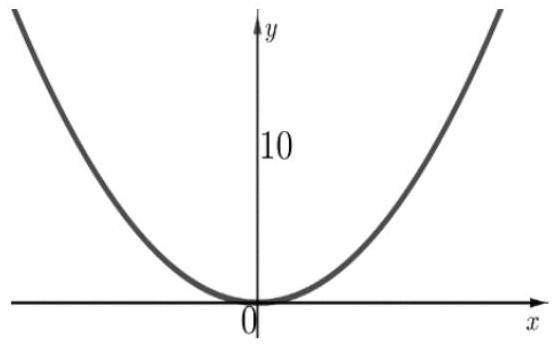
\includegraphics[scale=0.25]{ebe38402-76e9-4b46-a033-b1efc954d7e7-2_345_556_1165_1370}
	\end{minipage}
	\begin{corrBox}
		$x^2\leqslant5 \iff x\leqslant\sqrt{5}$ et $x\geqslant-\sqrt{5}$ car la fonction carré est décroissante sur $\R^-$ et renverse l'ordre.		
	\end{corrBox}
	
	\item Proposition 3 : L'inéquation $5-4 x \leqslant 3 x-6$ a pour ensemble solution dans $\mathbb{R}$ :
	\begin{multicols}{2}
		\begin{enumMet}
		\item $\left]-\infty ; \dfrac{11}{7}\right]$ 
		\item $\left.]-\infty ;-\dfrac{11}{7}\right]$
		\item \fbox{$\left[\dfrac{11}{7} ;+\infty\right[$}
		\item $\left[1 ;+\infty[\right.$
	\end{enumMet}
	\end{multicols}
	\begin{corrBox}
		$5-4 x \leqslant 3 x-6\iff 5+6\leqslant 3x+4x\iff 11\leqslant7x \iff \dfrac{11}{7}\leqslant x $
		
		Les solutions de l'inéquation sont donc tous les nombres supérieurs ou égal à $\dfrac{11}{7}$	
	\end{corrBox}
	\item Proposition 4 : L'expression affine $\mathrm{A}(x)=-2 x+8$ a pour tableau de signes :
	\begin{multicols}{2}
		\begin{enumMet}
			\item \begin{tikzpicture}
				\tkzTabInit[lgt = 1.5, espcl = 1.7]{$x$ / 1 , $A(x)$ / 1}{$-\infty$, $4$, $+\infty$}
				\tkzTabLine{, +, z, -, }
			\end{tikzpicture}	
			\item \begin{tikzpicture}
				\tkzTabInit[lgt = 1.5, espcl = 1.7]{$x$ / 1 , $A(x)$ / 1}{$-\infty$, $4$, $+\infty$}
				\tkzTabLine{, -, z, +, }
			\end{tikzpicture}	
			\item \begin{tikzpicture}
				\tkzTabInit[lgt = 1.5, espcl = 1.7]{$x$ / 1 , $A(x)$ / 1}{$-\infty$, $-4$, $+\infty$}
				\tkzTabLine{, +, z, -, }
			\end{tikzpicture}	
			\item \begin{tikzpicture}
				\tkzTabInit[lgt = 1.5, espcl = 1.7]{$x$ / 1 , $A(x)$ / 1}{$-\infty$, $-4$, $+\infty$}
				\tkzTabLine{, -, z, +, }
			\end{tikzpicture}	
		\end{enumMet}
	\end{multicols}
	\begin{corrBox}
		On résout $A(x)=0\iff -2x+8=0\iff -2x=-8\iff x=\dfrac{-8}{-2}=4$. De plus la fonction $A(x)$ est une fonction affine avec m<0 (coefficient directeur). Elle est donc strictement décroissante et d'abord positive et ensuite négative. Elle change de signe pour x=4. Solution a
		
		\begin{tikzpicture}
			\tkzTabInit[lgt = 1.5, espcl = 1.7]{$x$ / 1 , $A(x)$ / 1}{$-\infty$, $4$, $+\infty$}
			\tkzTabLine{, +, z, -, }
		\end{tikzpicture}	
	\end{corrBox}
	\item Proposition 5 : On considère la fonction $f$ définie sur $\mathbb{R}$ par $f(x)=25 x^{2}-81$. La forme factorisée de $f(x)$ est:
	\begin{multicols}{2}
		\begin{enumMet}
			\item 	$(5 x-9)^{2}$
			\item $(25 x-81)(25 x+81)$
			\item $5(x-9)^{2}$
			\item \fbox{$(5 x-9)(5 x+9)$}
		\end{enumMet}
	\end{multicols}
	\begin{corrBox}
		On reconnait la 3ème identité remarquable : $a^2-b^2=(a-b)(a+b)$
		
		$f(x)=25 x^{2}-81=(5x)^2-9^2=(5x-9)(5x+9)$		
	\end{corrBox}
	\item Proposition 6 : on a représenté ci-dessous une droite $\mathcal{D}$ dans un repère orthonormé.
%	\begin{center}
%		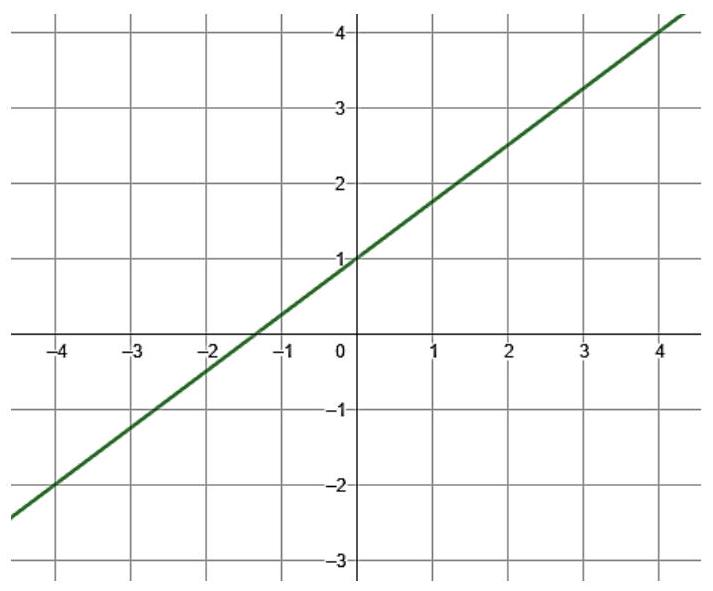
\includegraphics[scale=0.35]{ebe38402-76e9-4b46-a033-b1efc954d7e7-3_591_713_319_114}
%	\end{center}
	\begin{center}
		\begin{tikzpicture}%
			[x=0.7cm,y=0.7cm, %unités
			xmin=-5,xmax=5,xgrille=1,xgrilles=1, %axe Ox
			ymin=-3,ymax=4,ygrille=1,ygrilles=1] %axe Oy
			\GrilleTikz
			\AxesTikz%
			
			\AxexTikz[Police=\small]{-5,-4,...,5}
			\AxeyTikz[Police=\small]{-3,-2,...,4}
			\CourbeTikz[line width=1.4pt,ForestGreen,samples=250]%
			{-2/3*\x+1}{-4.45:5.05} %courbe
		\end{tikzpicture}
	\end{center}
	Une équation de la droite $\mathcal{D}$ est :
	\begin{multicols}{2}
		\begin{enumMet}
			\item \fbox{$y=-\dfrac{2}{3} x+1$}
			\item $y=\dfrac{2}{3} x+1$
			\item $2 x-3 y+1=0$
			\item $y=-\dfrac{3}{2} x+1$
		\end{enumMet}
	\end{multicols}
	\begin{corrBox}
		La droite passe par le point de coordonnées $(0;1)$ donc son ordonnée à l'origine $p=1$.
		
		Le coefficient directeur $m$ se lit graphiquement grâce à la méthode en escalier. Pour passer d'un point de la droite à un autre point, on se déplace de 3 unités vers la droite et 2 unités vers le bas donc $m=\dfrac{-2}{3}=-\dfrac{2}{3}$		
	\end{corrBox}
	
\end{enumMet}

\exerciceDS{ $-$ (05 points)}
Un particulier souhaite construire une terrasse rectangulaire et l'entourer d'une barrière sur 3 des côtés, le 4ème côté étant la maison. Par souci d'économie, il récupère du bois et commence par réaliser la barrière avant de faire sa terrasse. Avec le bois qu'il possède, il ne peut faire qu'un maximum de 32 m pour la barrière. On appelle $x$ la longueur du côté de la barrière perpendiculaire au mur de la maison.\\
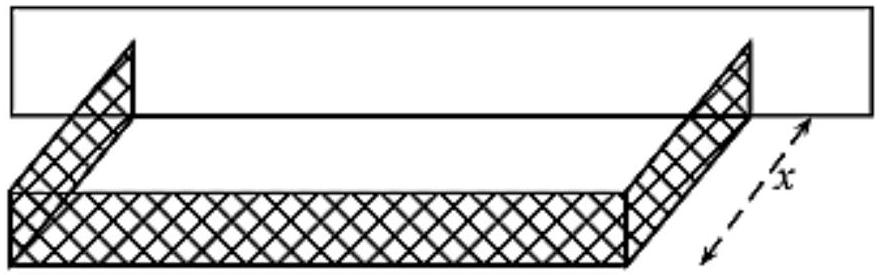
\includegraphics[scale=0.2]{ebe38402-76e9-4b46-a033-b1efc954d7e7-4_275_883_724_605}

On appelle $\mathcal{A}$ la fonction qui à un nombre $x$ associe $\mathcal{A}(x)$ l'aire de la terrasse.\\
La fonction $\mathcal{A}$ est ainsi définie sur l'intervalle [0;16].

\begin{enumMet}
	\item \begin{enumMet}
		\item Vérifier que l'aire $\mathcal{A}(x)=-2 x^{2}+32 x$.
		\begin{corrBox}
			$\mathcal{A}=\text{longueur}\times \text{largeur}=x(32-2x)=32x-2x^2=-2x^2+32x$		
		\end{corrBox}
		\item Montrer que la forme canonique de $\mathcal{A}(x)$ est $-2(x-8)^{2}+128$.
		\begin{corrBox}
			$\mathcal{A}(x)=-2 x^{2}+32 x=-2(x^2-16x)=-2(x^2-2x\times 8+8^2-8^2)=-2((x-8)^2-64)=-2(x-8)^2-2\times (-64)=-2(x-8)^2+128$		
		\end{corrBox}
	\end{enumMet}
	\item Quatre courbes ont été tracées sur le graphique ci-dessous. Identifier celle qui représente la fonction $\mathcal{A}$.
	\begin{center}
		\begin{tikzpicture}%
			[x=0.16cm,y=0.04cm, %unités
			xmin=0,xmax=100,xgrille=10,xgrilles=5, %axe Ox
			ymin=0,ymax=150,ygrille=10,ygrilles=10] %axe Oy
			\GrilleTikz
			\AxesTikz%
			\AxexTikz[Police=\small]{0,10,...,100}
			\AxeyTikz[Police=\small]{0,10,...,150}
			\CourbeTikz[line width=1.4pt,ForestGreen,samples=250]%
			{-2*(\x-8)^2+128}{0:16} %courbe
			\draw (15,120) node[color=ForestGreen] {$C_1$};
			\CourbeTikz[line width=1.4pt,red,samples=250]%
			{2*(\x-8)^2+128}{4.8:11.2} %courbe
			\draw (15,140) node[color=red] {$C_2$};
			\CourbeTikz[line width=1.4pt,blue,samples=250]%
			{-1.5*(\x-50)^2+90}{42.25:57.75} %courbe
			\draw (50,95) node[color=blue] {$C_3$};
			\CourbeTikz[line width=1.4pt,violet,samples=250]%
			{2*(\x-80)^2+8}{71.6:88.4} %courbe
			\draw (80,20) node[color=violet] {$C_4$};
			
		\end{tikzpicture}
	\end{center}
	\begin{corrBox}
		D'après la forme canonique, on sait que $\alpha=8$ et $\beta=128$. Le sommet de la parabole est donc le point de coordonnées $(\alpha; \beta)=(8;128)$.
		
		De plus $a=-2<0$ donc la courbe est une parabole tournée vers le bas.
		
		Il s'agit donc de la courbe $C_1$. 		
	\end{corrBox}
%	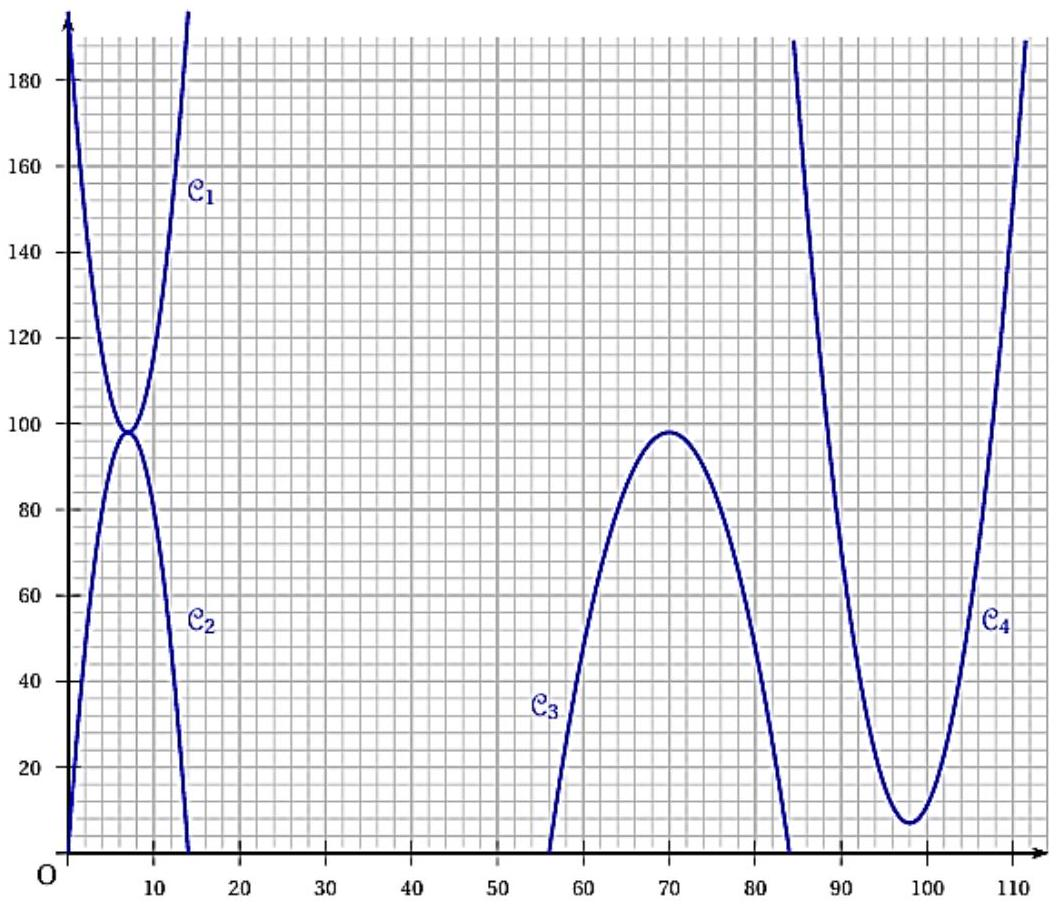
\includegraphics[scale=0.35]{ebe38402-76e9-4b46-a033-b1efc954d7e7-4_906_1056_1491_502}
	\item Dresser le tableau de variations de la fonction $\mathcal{A}$.
	\begin{corrBox}
		\begin{tikzpicture}
			\tkzTabInit{$x$ / 1 , $\mathcal{A}(x)$ / 1.5}{$0$, $8$, $16$}
			\tkzTabVar{-/ , +/ $128$, -/ }
		\end{tikzpicture}		
	\end{corrBox}
	\item Pour quelle valeur de $x$ l'aire de la terrasse est-elle maximale ? Donner la valeur de cette aire.
	\begin{corrBox}
		L'aire maximale est de $128\ m^2$ quand $x=8\ m$		
	\end{corrBox}
	\item Pour quelles valeurs de $x$ l'aire de la terrasse est-elle supérieure ou égale à $96 \mathrm{~m}^{2}$ ?
	\begin{corrBox}
		On résout l'inéquation $-2x^2+32x\geqslant 96$ 
		
		$-2x^2+32x\geqslant 96\iff -2x^2+32x-96\geqslant 0$
		
		$\Delta=32^2-4\times 2\times 96=256=16$
		
		$x_1=\dfrac{-32-4}{-4}=9$ et $x_2=\dfrac{-32+4}{-4}=7$	
		
		\begin{tikzpicture}
			\tkzTabInit{$x$ / 1 , $-2x^2+32x-96$ / 1}{$0$, $7$,$9$ ,$16$}
			\tkzTabLine{, -, z, +, z, -,}
		\end{tikzpicture}
		
		L'aire de la terrasse est supérieure ou égale à $96m^2$ quand x est compris entre 7 et 9 m.	
	\end{corrBox}
\end{enumMet}

\exerciceDS{ $-$ (04 points)}
On considère la fonction $f$ définie sur $[0 ; 5 \pi]$ par $f(x)=2 \sin \left(\dfrac{x+2\pi}{2}\right)$.\\
La courbe représentative $\left(\mathcal{C}_{f}\right)$ de la fonction $f$ est représentée dans le repère ci-dessous:
\begin{center}
	\begin{tikzpicture}[x=1cm,y=1.2cm,xmin=0,xmax={5*pi},xgrille=0.5,xgrilles=0.25,
		ymin=-2.5,ymax=2.5,ygrille=0.5,ygrilles=0.25]
		\GrilleTikz \AxesTikz
		\AxexTikz[Trigo]{{pi/3},{2*pi/3},{pi},{4*pi/3},%
			{5*pi/3},{2*pi},{7*pi/3},{8*pi/3},{3*pi},{10*pi/3},{11*pi/3},{4*pi},{13*pi/3},{14*pi/3},{5*pi}}
		\AxeyTikz[Police=\small]{-2,-1,...,2}
		\CourbeTikz[thick,blue,samples=250]{2*sin(deg((\x+2*pi)/2)}{0:5*pi}
	\end{tikzpicture}
\end{center}
%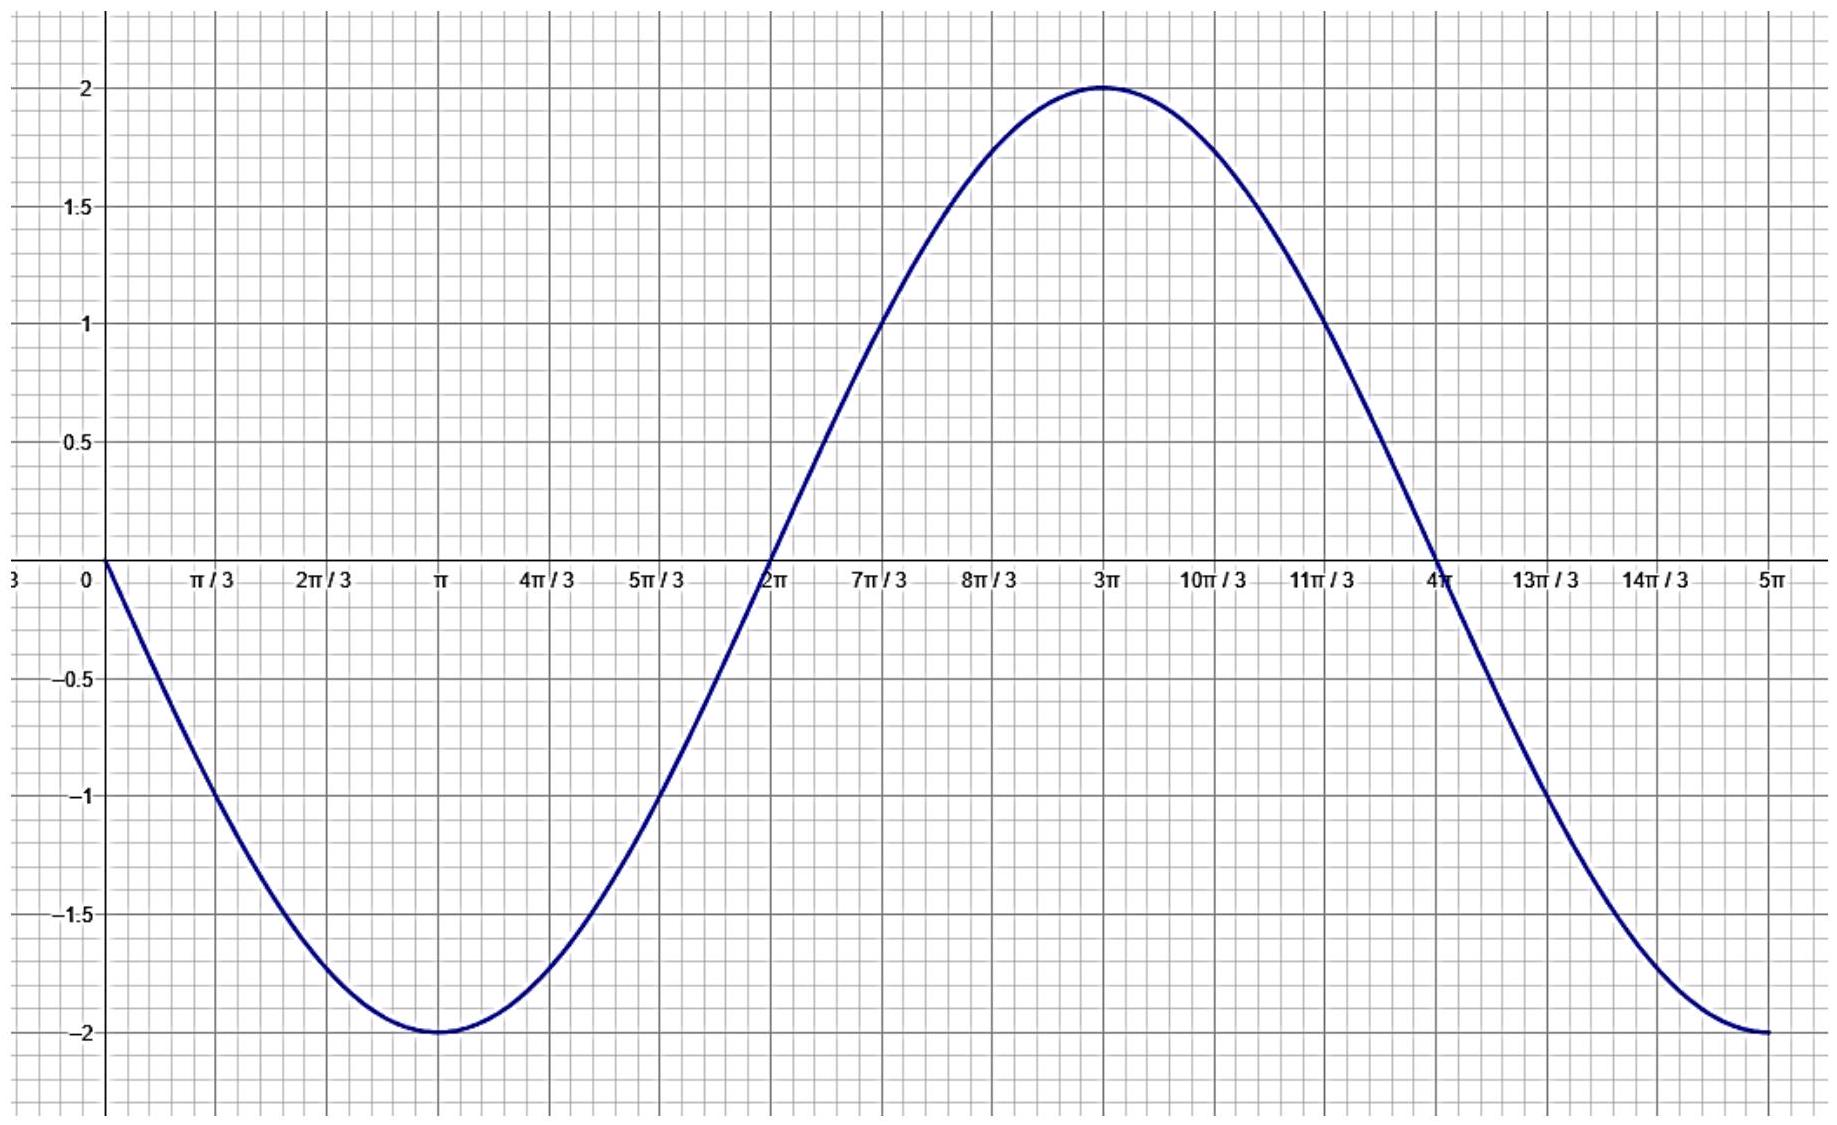
\includegraphics[scale=0.26]{ebe38402-76e9-4b46-a033-b1efc954d7e7-5_1125_1837_559_114}

\subsection*{Partie A: lectures graphiques}
Avec la précision permise par le graphique,

\begin{enumMet}
	\item Déterminer l'encadrement le plus précis possible de $f(x)$.
	\begin{corrBox}
		Le maximum de la fonction semble être 2 et le minimum $-2$. Donc $-2\leqslant f(x)\leqslant 2$.		
	\end{corrBox}
	\item Déterminer l'image de $\dfrac{10 \pi}{3}$ par la fonction $f$.
	\begin{corrBox}
		$f\left(\dfrac{10 \pi}{3}\right)\approx1,75$	
	\end{corrBox}
	\item Déterminer le(s) antécédent(s) de 1 par la fonction $f$.
	\begin{corrBox}
		Les antécédents de 1 par la fonction f sont :$\dfrac{7\pi}{3}$ et $\dfrac{11\pi}{3}$.		
	\end{corrBox}
\end{enumMet}

\subsection*{Partie B : justifications mathématiques}
\begin{enumMet}
	\item Démontrer que, pour tout $x$ de l'intervalle $[0 ; 5 \pi]$, on a $-2 \leqslant f(x) \leqslant 2$.
	\begin{corrBox}
		pour tout $x$ de l'intervalle $[0 ; 5 \pi]$ on a $-1\leqslant \sin(x)\leqslant 1$
		donc $-1\leqslant \sin \left(\dfrac{x+2\pi}{2}\right)\leqslant 1$
		soit finalement $-2\leqslant 2\sin \left(\dfrac{x+2\pi}{2}\right)\leqslant 2$ et donc $-2\leqslant f(x)\leqslant 2$	
	\end{corrBox}
	\item \begin{enumMet}
		\item Déterminer, en expliquant votre démarche, la mesure principale de $\dfrac{8 \pi}{3}$.
		\begin{corrBox}
			$\dfrac{8 \pi}{3}=\dfrac{6 \pi}{3}+\dfrac{2\pi}{3}=2\pi+\dfrac{2\pi}{3}$.
			
			La mesure principale de l'angle est donc $\dfrac{2\pi}{3}$		
		\end{corrBox}
		\item En déduire la valeur exacte de $f\left(\dfrac{10 \pi}{3}\right)$.
		\begin{corrBox}
			$f\left(\dfrac{10 \pi}{3}\right)=2\sin \left(\dfrac{\frac{10\pi}{3}+2\pi}{2}\right)=2\sin \left(\dfrac{\frac{16\pi}{3}}{2}\right)=2\sin \left(\dfrac{16\pi}{6}\right)$
			
			$f\left(\dfrac{10 \pi}{3}\right)=2\sin \left(\dfrac{8\pi}{3}\right)=2\sin \left(\dfrac{2\pi}{3}\right)=2\times \dfrac{\sqrt{3}}{2}=\sqrt{3}$		
		\end{corrBox}
	\end{enumMet}
	\item \begin{enumMet}
		\item En s'appuyant sur un cercle trigonométrique, résoudre l'équation $\sin (X)=\dfrac{1}{2}$ dans l'intervalle $\left[\pi ; 3 \pi\right]$
		\begin{corrBox}
			$\sin (X)=\dfrac{1}{2} \iff S=\left\{\dfrac{13\pi}{6};\dfrac{17\pi}{6}(2\pi)\right\}$		
		\end{corrBox}
		\item En déduire les solutions de l'équation $f(x)=1$ dans l'intervalle $[0 ; 5 \pi]$.
		\begin{corrBox}
			S1 : $\dfrac{x+2\pi}{2}=\dfrac{\pi}{6}\iff 3x+6\pi=13\pi \iff x=\dfrac{7\pi}{3}$
			
			S2 : $\dfrac{x+2\pi}{2}=\dfrac{5\pi}{6}\iff 3x+6\pi=17\pi \iff x=\dfrac{11\pi}{3}$
			
			On retrouve les valeurs trouvés graphiquement dans la partie A. 		
		\end{corrBox}
	\end{enumMet}
\end{enumMet}

\newpage
\exerciceDS{ $-$ (05 points)}
Dans le plan muni d'un repère orthonormé ( $O ; \vec{\imath}, \vec{\jmath}$ ), on considère les points $A(-1 ; 5), B(-7 ; -3)$ et $C(7 ;-1)$.

Données : $\sqrt{50}=5 \sqrt{2}$ et $\dfrac{1}{\sqrt{2}}=\dfrac{\sqrt{2}}{2}$

\begin{enumMet}
	\item Tracer le triangle $A B C$ dans le repère donné ci-dessous :
	
%	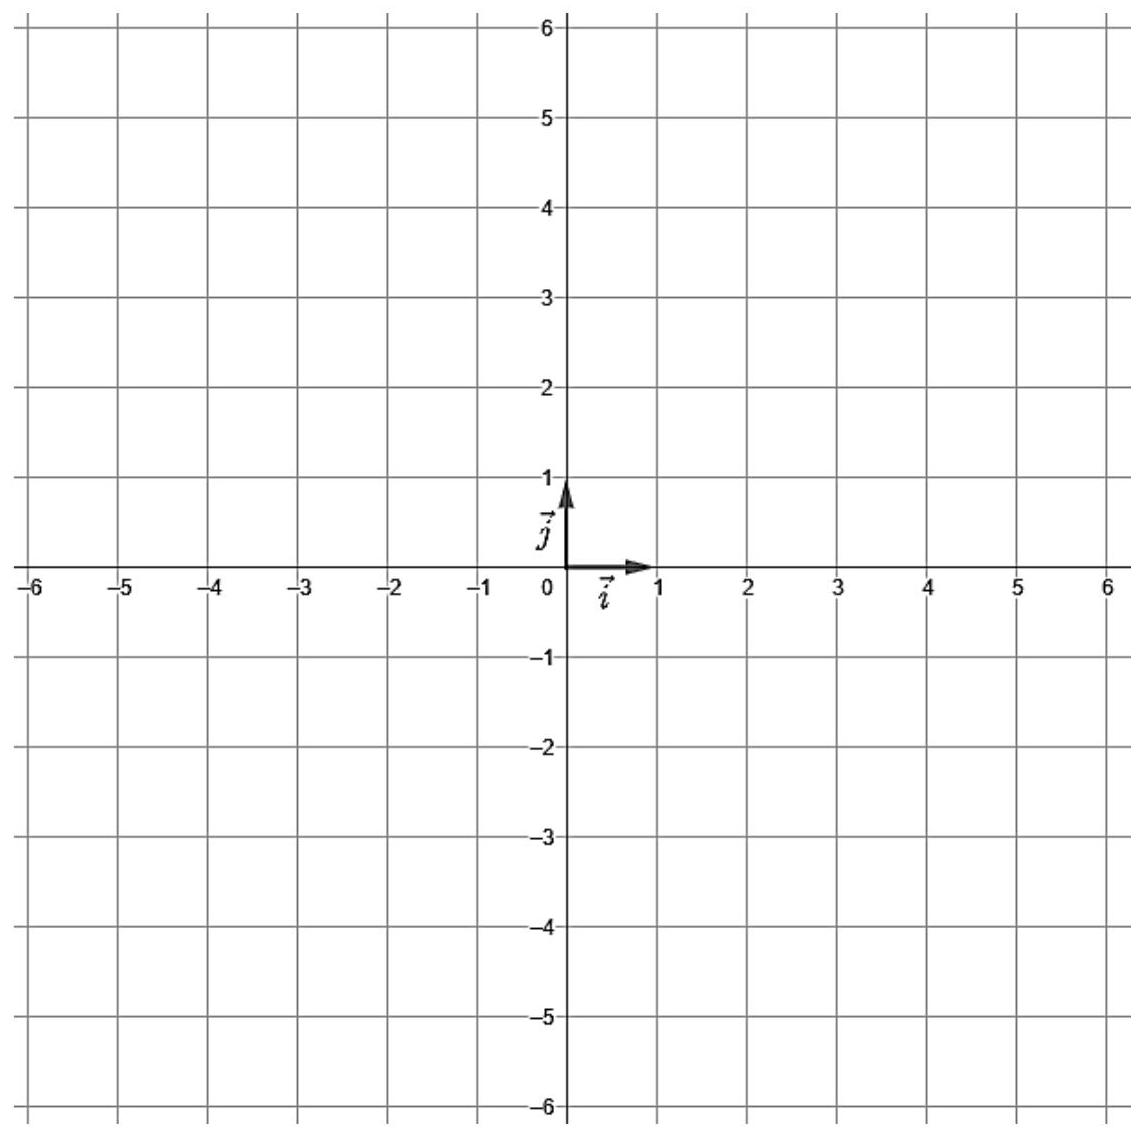
\includegraphics[scale=0.35]{ebe38402-76e9-4b46-a033-b1efc954d7e7-6_1137_1143_794_461}
	\begin{center}
		\begin{tikzpicture}%
			[x=1cm,y=1cm, %unités
			xmin=-8,xmax=8,xgrille=1,xgrilles=1, %axe Ox
			ymin=-4,ymax=6,ygrille=1,ygrilles=1] %axe Oy
			\GrilleTikz
			\AxesTikz%
			
			\AxexTikz[Police=\small]{-8,-7,...,8}
			\AxeyTikz[Police=\small]{-4,-3,...,6}
%			\CourbeTikz[line width=1.4pt,ForestGreen,samples=250]%
%			{-2/3*\x+1}{-4.45:5.05} %courbe
			\coordinate (A) at (-1,5);
			\coordinate (B) at (-7,-3);
			\coordinate (C) at (7,-1);
			\node at (A) {$\bullet$};
			\node at (B) {$\bullet$};
			\node at (C) {$\bullet$};
			\draw [red] (A) to (B);
			\draw [red] (A) to (C);
			\draw [red] (B) to (C);
			\draw (A) node[red,above]{$A$};
			\draw (B) node[red,left]{$B$};
			\draw (C) node[red,right]{$C$}; 
		\end{tikzpicture}
	\end{center}
	\item Calculer le produit scalaire $\vv{B C} \cdot \vv{B A}$.
	\begin{corrBox}
		On commence par calculer les coordonnées de $\vv{B C}$ et $\vv{B A}$.
		
		$\Coord{BC}{x_C-x_B}{y_C-y_B}=\Coord{BC}{7-(-7)}{-1-(-3)}=\Coord{BC}{14}{2}$
		
		$\Coord{BA}{x_A-x_B}{y_A-y_B}=\Coord{BA}{-1-(-7)}{5-(-3)}=\Coord{BA}{6}{8}$
		
		$\vv{B C} \cdot \vv{B A}=xx'+yy'=14\times 6+8\times 2=100$		
	\end{corrBox}
	\item \begin{enumMet}
		\item Exprimer $\vv{B C} \cdot \vv{B A}$ en fonction de l'angle ( $\vv{B C} ; \vv{B A}$ ).
		\begin{corrBox}
			$\vv{B C} \cdot \vv{B A}=BC\times BA\times \cos( \vv{B C} ; \vv{B A} )$		
		\end{corrBox}
		\item En déduire la valeur exacte de l'angle orienté ( $\vv{B C} ; \vv{B A}$ ) en radians.
		\begin{corrBox}
			$BC=\sqrt{14^2+2^2}=\sqrt{200}=10\sqrt{2}$
			
			$BA=\sqrt{6^2+8^2}=\sqrt{100}=10$
			
			$\vv{B C} \cdot \vv{B A}=BC\times BA\times \cos( \vv{B C} ; \vv{B A} )$
			$\iff 100=10\sqrt{2}\times 10\times \cos( \vv{B C} ; \vv{B A} )$
			$\iff \cos( \vv{B C} ; \vv{B A} )=\dfrac{100}{10\sqrt{2}\times 10}=\dfrac{1}{\sqrt{2}}=\dfrac{\sqrt{2}}{2}$
			
			d'ou $( \vv{B C} ; \vv{B A} )=\dfrac{\pi}{4}$		
		\end{corrBox}
	\end{enumMet}
	\item Montrer que le triangle $A B C$ est rectangle, et préciser en quel point.
	\begin{corrBox}
		On peut faire la réciproque de pythagore en calculant la troisième longueur (AC) ou faire avec le produit scalaire $\vv{AB} \cdot \vv{AC}$.
		
		Comme $\vv{AB}=-\vv{BA}$ on a $\Coord{AB}{-6}{-8}$
		
		$\Coord{AC}{x_C-x_A}{y_C-y_A}=\Coord{AC}{7-(-1)}{-1-5}=\Coord{AC}{8}{-6}$
		
		$\vv{AB} \cdot \vv{AC}=xx'+yy'=-6\times 8+6\times 8=0$.
		
		Les vecteurs $\vv{AB}$ et $\vv{AC}$ sont orthogonaux donc les droites (AB) et (AC) sont perpendiculaires. Le triangle ABC est donc rectangle en A.		
	\end{corrBox}
	\item \begin{enumMet}
		\item Calculer les longueurs $A B$ et $A C$.
		\begin{corrBox}
			$AB=BA=\sqrt{6^2+8^2}=\sqrt{100}=10$
			
			$AC=\sqrt{8^2+(-6)^2}=\sqrt{64+36}=\sqrt{100}=10$		
		\end{corrBox}
		\item En déduire la valeur exacte de l'angle orienté $(\vv{C B} ; \vv{C A})$ en radians.
		\begin{corrBox}
			On a AB=AC, donc le triangle ABC est rectangle et isocèle en A, on a donc :
			
			$(\vv{C B} ; \vv{C A})=( \vv{B C} ; \vv{B A} )=\dfrac{\pi}{4}$ 		
		\end{corrBox}
	\end{enumMet}
\end{enumMet}



\end{document}

